%% LaTeX-Beamer template for KIT design
%% by Erik Burger, Christian Hammer
%% title picture by Klaus Krogmann
%%
%% version 2.1
%%
%% mostly compatible to KIT corporate design v2.0
%% http://intranet.kit.edu/gestaltungsrichtlinien.php
%%
%% Problems, bugs and comments to
%% burger@kit.edu

\documentclass[18pt]{beamer}

%% SLIDE FORMAT

% use 'beamerthemekit' for standard 4:3 ratio
% for widescreen slides (16:9), use 'beamerthemekitwide'

\usepackage{templates/beamerthemekit}
\usepackage[utf8]{inputenc}
\usepackage[T1]{fontenc}
\usepackage{graphicx}
% \usepackage{templates/beamerthemekitwide}

%% TITLE PICTURE

% if a custom picture is to be used on the title page, copy it into the 'logos'
% directory, in the line below, replace 'mypicture' with the 
% filename (without extension) and uncomment the following line
% (picture proportions: 63 : 20 for standard, 169 : 40 for wide
% *.eps format if you use latex+dvips+ps2pdf, 
% *.jpg/*.png/*.pdf if you use pdflatex)

%\titleimage{mypicture}

%% TITLE LOGO

% for a custom logo on the front page, copy your file into the 'logos'
% directory, insert the filename in the line below and uncomment it

%\titlelogo{mylogo}

% (*.eps format if you use latex+dvips+ps2pdf,
% *.jpg/*.png/*.pdf if you use pdflatex)

%% TikZ INTEGRATION

% use these packages for PCM symbols and UML classes
% \usepackage{templates/tikzkit}
% \usepackage{templates/tikzuml}

% the presentation starts here

\title{Themenvorschläge der Java-Gruppe}
\subtitle{Netzwerksimulator Sinalgo oder Neuronale Netze mit Neuroph}
\author{Markus Braun, Daniel Hammann, Dominik Messinger, Dominic Rausch}

\institute{Institut für Programmstrukturen und Datenorganisation (IPD), Lehrstuhl für Programmiersysteme}

% Bibliography

%\usepackage[citestyle=authoryear,bibstyle=numeric,hyperref,backend=biber]{biblatex}
%\addbibresource{templates/example.bib}
%\bibhang1em

\begin{document}
	\maketitle

	\begin{frame}[c]\frametitle{Sinalgo\footnote{http://disco.ethz.ch/projects/sinalgo/} }
		\begin{block}{}
			\begin{itemize}
			\item Netzwerksimulator von der ETH Zürich
			\item Features
			\begin{itemize}
				\item Bewegliche Knotenpunkte
				\item Eigenes Verbindungsmodel
				\item Eigenes Interferenz- und Verlässlichkeitsmodel
				\item Übertragungszeit
			\end{itemize}
			\item \textbf{Langsam!}
			\end{itemize}
		\end{block}
	\end{frame}

	\begin{frame}[c]\frametitle{Sinalgo - Was ist zu tun?}
		\begin{block}{Status Quo}
		    \begin{itemize}
		    	\item Ein Thread
		    	\item Mehrfache Iteration über jeden Knoten
		    	\item Asynchron und Synchron Modus
		    \end{itemize}
		\end{block}
		\begin{block}{Herausforderungen}
			\begin{itemize}
		    	\item Nebenläufiges Verschieben und Neuverbinden der Knoten
		    	\item Nebenläufige Simulation des Knotenverhaltens
		    	\item Evtl: Anpassung der GUI nötig
		    \end{itemize}
		\end{block}
	\end{frame}
	
	\begin{frame}[c]\frametitle{Neuroph\footnote{http://neuroph.sourceforge.net/}}
		\begin{block}{}
		\begin{itemize}
			\item Künstliches Neuronales Netz - Framework in Java
			\item Features
			\begin {itemize}
				\item leichtgewichtiges, intuitives Framework
				\item unterstützt verschiedene ANNs, z.B. Multi Layer Perzeptron mit Backpropagation
				\item Anwendungen sind Klassifikations-, Erkennungsaufgaben, Vorhersagen...
			\end {itemize}
			\item versteckte Schicht mit 500 Neuronen $\rightarrow$ \textbf{47s!}
		\end {itemize}
		\end{block}
		\begin{center}
		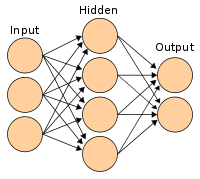
\includegraphics[scale=0.4]{ann.png}
		\end{center}
	\end {frame}
	
	\begin{frame}[c]\frametitle{Neuroph - Was ist zu tun?}
		\begin{block}{Status Quo}
		    \begin{itemize}
		    	\item Ein Thread pro komplettes Traning-Set
		    	\item MLP: Iteration über Layer, pro Layer wiederum Iteration über Neuronen
		    	\item große Schicht führt unmittelbar zu langer Laufzeit
		    \end{itemize}
		\end{block}
		\begin{block}{Herausforderungen}
		    \begin{itemize}
		    	\item Nebenläufiges Trainieren und Anwenden: Schichten aufteilen und parallel berechnen
		    \end{itemize}
		\end{block}
	\end{frame}

\end{document}